\begin{frame}{MC efficiency (1)}
\setlength{\unitlength}{1mm}
\begin{center}
MC true events $\chi_b(3P) \to \Y1S \gamma$ (other decays have the same shape)
\begin{picture}(70,50)
      %
    \put(0,0){
      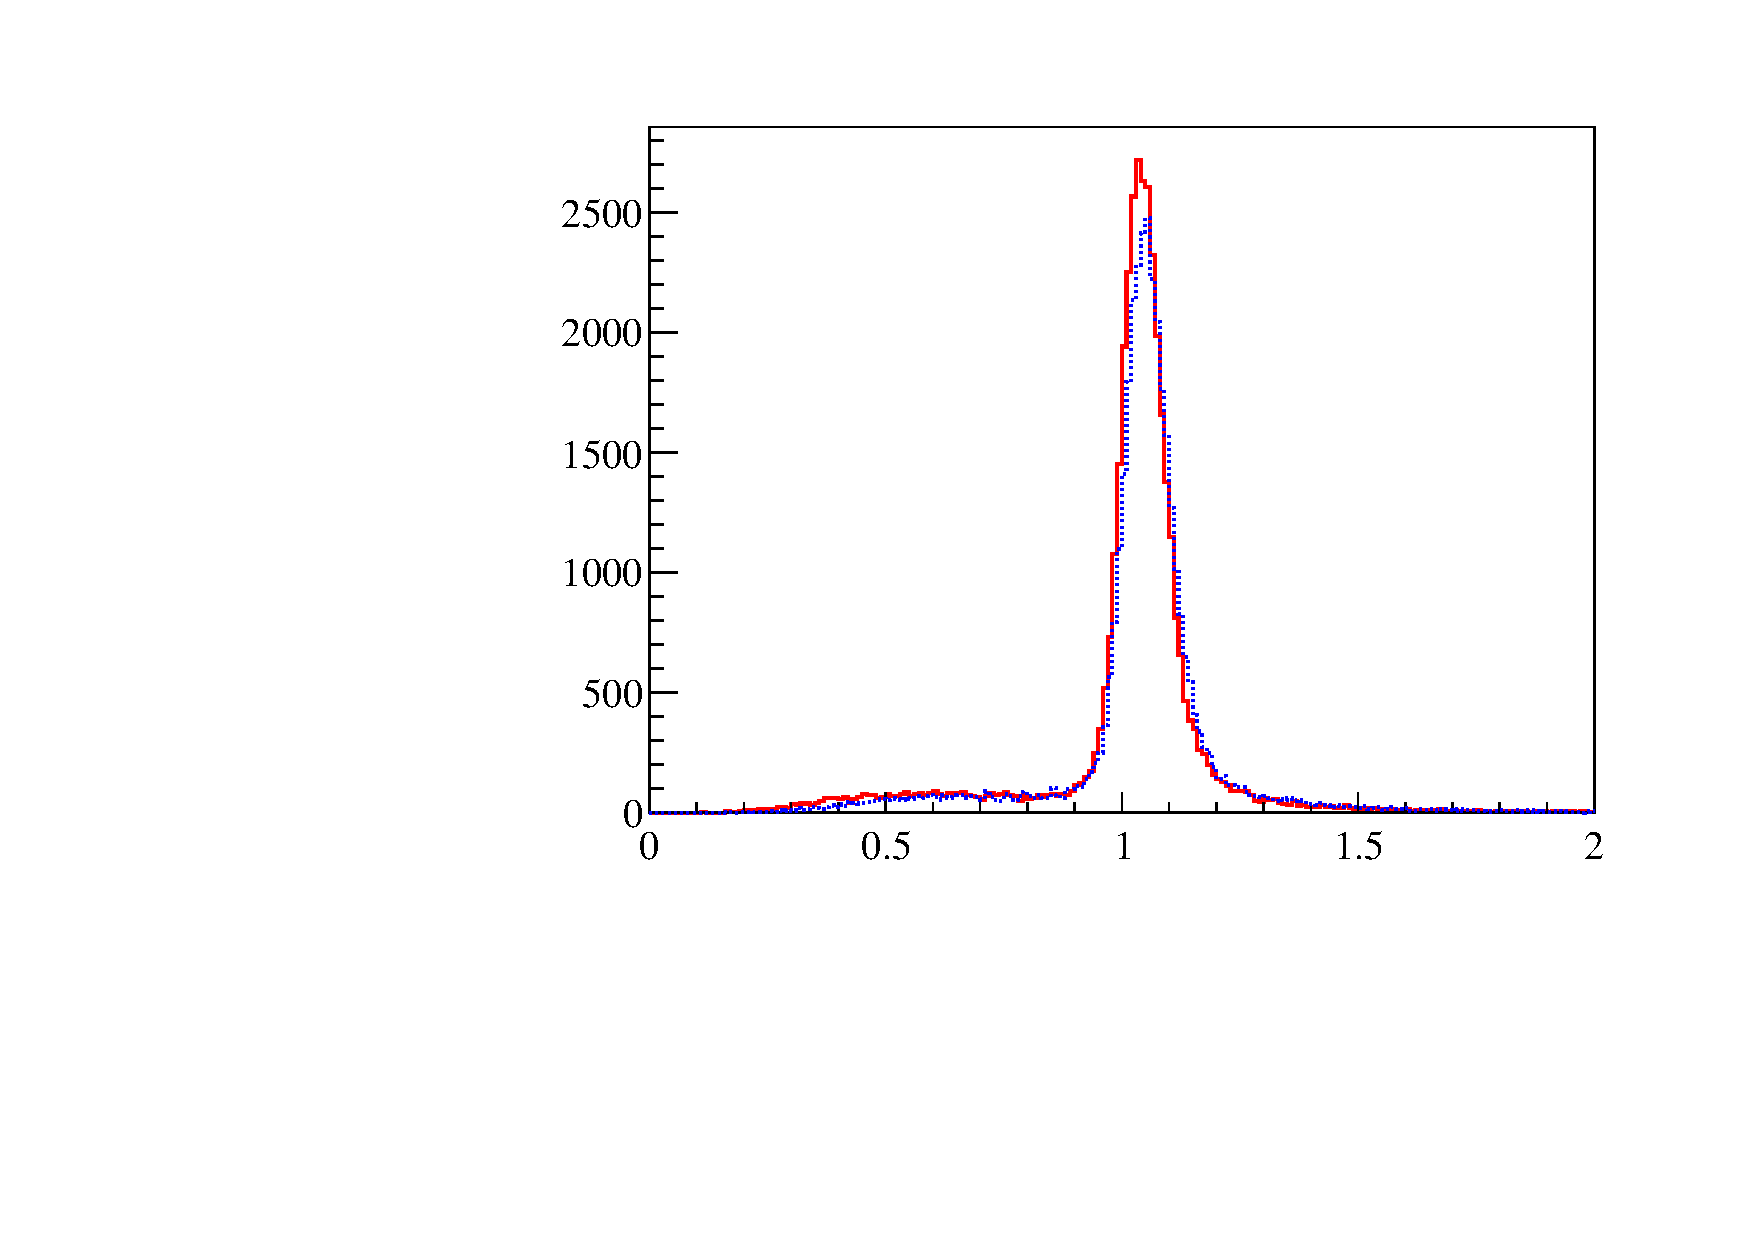
\includegraphics[width=70mm, height=50mm]{mc-fits/cb3_h}
    }
    
%    \put(0,40){
%      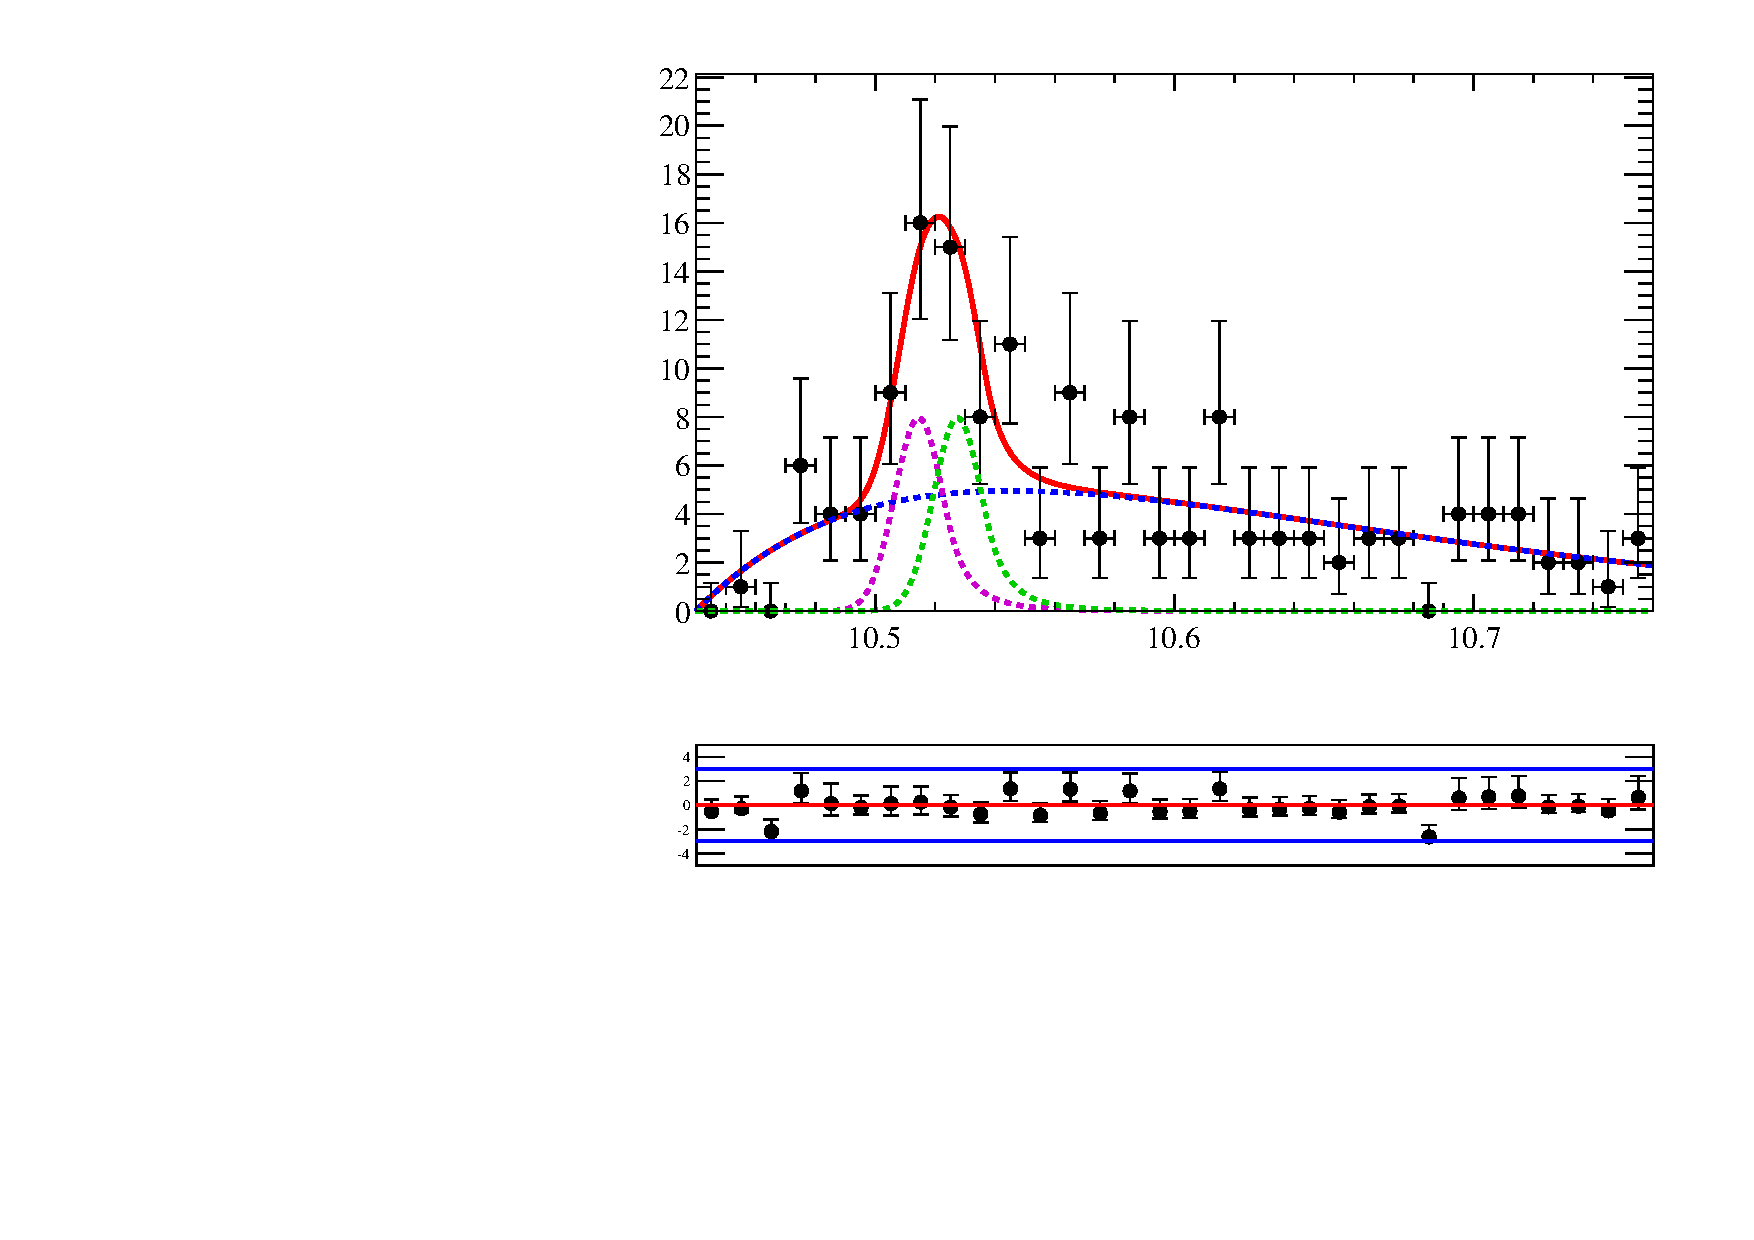
\includegraphics[width=50mm, height=40mm]{7.1-chib3s-fit/f2011_fix_27_None}
%    }

    \put(0,12){\begin{sideways}Candidates\end{sideways}}
    \put(20,0){$m_{\mumu \gamma} - m_{\mumu} \left[\gevcc\right]$}

%    
%    \put(0,55){\tiny \begin{sideways}Candidates/(20\mevcc)\end{sideways}}
%    \put(2, 49.5){\tiny $m_{\mumu \gamma} - m_{\mumu} + 10.3552 \left[\gevcc\right]$}
%    \put(25,70){$\sqrt{s} = 7 \gev$}     
%    \graphpaper[2](0,0)(70, 50)        
  \end{picture}
 \end{center}
 
\begin{alertblock}{}
Monte-Carlo events in the flat left band are fitted as
background in the model for real data. So efficiency needs to be calculated with \chib mc-true events fitted by Crystal Ball function and some background which fits this band. 
$\Upsilon$ events are measured by counting mc-true events.

\end{alertblock}

\end{frame}